\documentclass[11pt]{article}
\usepackage[margin=1in]{geometry}
\usepackage{listings,xcolor,hyperref,booktabs,longtable,tikz}
\usetikzlibrary{arrows.meta,positioning}
\lstset{basicstyle=\ttfamily\small,breaklines=true,frame=single,numbers=left,numberstyle=\tiny\color{gray}}
\title{Data Fabric Architecture:\\Federated MCP Mesh for Enterprise AI}
\author{SAP OSS Technical Documentation}
\date{March 2026}

\hypersetup{
  colorlinks=true,
  linkcolor=blue!70!black,
  urlcolor=blue!70!black,
  citecolor=blue!70!black
}

\newcommand{\filepath}[1]{\texttt{#1}}
\newcommand{\code}[1]{\texttt{#1}}

\begin{document}
\maketitle

\begin{abstract}
This document describes the Data Fabric architecture of the SAP OSS platform,
a federated Model Context Protocol (MCP) mesh that unifies LangChain,
SAP HANA Cloud vector stores, KuzuDB graph databases, and SAP AI Core
deployments behind a single JSON-RPC 2.0 surface.  The architecture spans
four primary subsystems: (1)~an MCP server with 11 registered tools and 3
resources backed by a Mangle fact store, (2)~a CAP LLM Plugin that
extends \code{cds.Service} with OpenTelemetry-instrumented embedding,
chat completion, RAG, and streaming operations, (3)~a KuzuDB Graph-RAG
layer that maintains entity relationships across HANA vector stores,
embedding deployments, and schema classifications, and (4)~an Angular
Fabric Console that provides browser-based MCP tool invocation, health
polling, and deployment management.  All code evidence references exact
file paths and line numbers from the repository.
\end{abstract}

\tableofcontents
\newpage

% ═══════════════════════════════════════════════════════════════════
\section{MCP Server Architecture}
\label{sec:mcp-server}
% ═══════════════════════════════════════════════════════════════════

The MCP server is implemented as a single-file Python HTTP server in
\filepath{src/data/langchain-integration-for-sap-hana-cloud-main/mcp\_server/server.py}.
It uses the standard library \code{http.server} module (line~12) rather than
a framework, yielding a zero-dependency deployment artifact.

\subsection{MCPServer Class}

The \code{MCPServer} class (line~288) is the central coordinator.  Its constructor
initializes three registries and configures federated endpoints:

\begin{lstlisting}[language=Python,caption={MCPServer constructor (server.py lines 289--305)},label=lst:mcpserver-init]
class MCPServer:
    def __init__(self):
        self.tools = {}
        self.resources = {}
        self.facts = {}
        self.local_mcp_endpoint = normalize_mcp_endpoint(
            os.environ.get("LANGCHAIN_MCP_ENDPOINT",
              f"http://localhost:{os.environ.get('MCP_PORT','9140')}/mcp")
        )
        self.hana_mcp_endpoint = normalize_mcp_endpoint(
            os.environ.get("LANGCHAIN_HANA_MCP_ENDPOINT",
              "http://localhost:9130/mcp")
        )
        self.odata_mcp_endpoint = normalize_mcp_endpoint(
            os.environ.get("LANGCHAIN_ODATA_MCP_ENDPOINT",
              "http://localhost:9150/mcp")
        )
        self.remote_mcp_endpoints = get_remote_mcp_endpoints(
            "LANGCHAIN_REMOTE_MCP_ENDPOINTS")
        self._register_tools()
        self._register_resources()
        self._initialize_facts()
\end{lstlisting}

\subsection{JSON-RPC 2.0 over HTTP}

The server exposes a single \code{POST /mcp} endpoint.  The HTTP handler
(\code{MCPHandler}, line~993) enforces request size limits
(\code{MAX\_REQUEST\_BYTES}, line~42, default 1\,MB), validates UTF-8 encoding,
and parses JSON-RPC payloads.  The \code{handle\_request} method (line~921)
dispatches on the \code{method} field:

\begin{itemize}
  \item \code{initialize} --- returns protocol version \code{2024-11-05} and
        capability declarations (line~933).
  \item \code{tools/list} --- enumerates registered tools (line~940).
  \item \code{tools/call} --- dispatches to the appropriate handler via a
        name-to-function map (lines~949--961).
  \item \code{resources/list} --- enumerates registered resources (line~968).
  \item \code{resources/read} --- reads resource content by URI (lines~971--977).
\end{itemize}

Protocol version validation occurs at line~927, rejecting requests where
\code{jsonrpc} is not \code{"2.0"} with error code \code{-32600}.

\subsection{Tool Registry (11 Tools)}

The \code{\_register\_tools} method (line~307) populates the tool registry with
11 tools.  Each tool definition follows the MCP tool schema with
\code{name}, \code{description}, and \code{inputSchema} fields.
Table~\ref{tab:tools} summarizes all registered tools.

\begin{longtable}{@{}llp{5.5cm}@{}}
\caption{Registered MCP tools (server.py lines 307--500)}
\label{tab:tools} \\
\toprule
\textbf{Tool Name} & \textbf{Lines} & \textbf{Purpose} \\
\midrule
\endfirsthead
\toprule
\textbf{Tool Name} & \textbf{Lines} & \textbf{Purpose} \\
\midrule
\endhead
\bottomrule
\endlastfoot
\code{langchain\_chat}                & 309--321  & Chat completion via LangChain + HANA \\
\code{langchain\_vector\_store}       & 324--335  & Create or retrieve HANA vector store \\
\code{langchain\_add\_documents}      & 338--350  & Add documents to HANA vector store \\
\code{langchain\_similarity\_search}  & 353--366  & Similarity search in HANA vector store \\
\code{langchain\_rag\_chain}          & 369--381  & Run RAG chain with HANA retriever \\
\code{langchain\_embeddings}          & 384--395  & Generate embeddings via LangChain \\
\code{langchain\_load\_documents}     & 398--409  & Load documents using LangChain loaders \\
\code{langchain\_split\_text}         & 412--424  & Sentence-aware recursive text splitting \\
\code{mangle\_query}                  & 427--438  & Query the Mangle reasoning engine \\
\code{kuzu\_index}                    & 441--476  & Index HANA entities into KuzuDB graph \\
\code{kuzu\_query}                    & 479--500  & Read-only Cypher query against KuzuDB \\
\end{longtable}

\subsection{Resource Registry (3 Resources)}

The \code{\_register\_resources} method (line~502) registers three MCP resources:

\begin{lstlisting}[language=Python,caption={Resource registration (server.py lines 502--520)},label=lst:resources]
def _register_resources(self):
    self.resources["langchain://vectorstores"] = {
        "uri": "langchain://vectorstores",
        "name": "Vector Stores",
        "description": "Available HANA vector stores",
        "mimeType": "application/json",
    }
    self.resources["langchain://chains"] = {
        "uri": "langchain://chains",
        "name": "Chains",
        "description": "Available LangChain chains",
        "mimeType": "application/json",
    }
    self.resources["mangle://facts"] = {
        "uri": "mangle://facts",
        "name": "Mangle Facts",
        "description": "Mangle fact store",
        "mimeType": "application/json",
    }
\end{lstlisting}

\subsection{Mangle Fact Store}

The \code{\_initialize\_facts} method (line~522) populates the Mangle fact store
with a \code{service\_registry} list containing all known MCP endpoints,
\code{tool\_invocation} for audit logging, and \code{vector\_stores} for tracking
active stores.  Remote endpoints from \code{LANGCHAIN\_REMOTE\_MCP\_ENDPOINTS}
are appended with model tag \code{"federated"} (lines~532--533).

\begin{lstlisting}[language=Python,caption={Fact store initialization (server.py lines 522--536)},label=lst:facts]
def _initialize_facts(self):
    self.facts["service_registry"] = [
        {"name": "langchain-mcp",
         "endpoint": self.local_mcp_endpoint,
         "model": "langchain-hana-mcp"},
        {"name": "hana-toolkit-mcp",
         "endpoint": self.hana_mcp_endpoint,
         "model": "hana-ai-toolkit-mcp"},
        {"name": "odata-vocab-mcp",
         "endpoint": self.odata_mcp_endpoint,
         "model": "odata-vocab-mcp"},
        ...
    ]
    for idx, endpoint in enumerate(self.remote_mcp_endpoints):
        self.facts["service_registry"].append(
            {"name": f"remote-mcp-{idx+1}",
             "endpoint": endpoint, "model": "federated"})
    self.facts["tool_invocation"] = []
    self.facts["vector_stores"] = []
\end{lstlisting}


% ═══════════════════════════════════════════════════════════════════
\section{Federated MCP Mesh}
\label{sec:federated-mesh}
% ═══════════════════════════════════════════════════════════════════

The federated mesh allows any MCP server instance to delegate tool calls
to peer servers.  This section details the three key functions that
enable federation.

\subsection{Priority-Ordered Endpoint Iteration}

The \code{\_iter\_federated\_mcp\_endpoints} method (line~537) constructs a
priority-ordered list of remote endpoints, deduplicating and filtering
out the local endpoint:

\begin{lstlisting}[language=Python,caption={Federated endpoint iteration (server.py lines 537--564)},label=lst:iter-federated]
def _iter_federated_mcp_endpoints(self, preferred=None):
    ordered = []
    seen = set()
    def push(endpoint):
        normalized = normalize_mcp_endpoint(endpoint)
        if not normalized:
            return
        if normalized == self.local_mcp_endpoint:
            return
        if not (normalized.startswith("http://")
                or normalized.startswith("https://")):
            return
        if normalized in seen:
            return
        seen.add(normalized)
        ordered.append(normalized)
    for endpoint in preferred or []:
        push(endpoint)
    for endpoint in self.remote_mcp_endpoints:
        push(endpoint)
    for service in self.facts.get("service_registry", []):
        if not isinstance(service, dict):
            continue
        endpoint = service.get("endpoint")
        if isinstance(endpoint, str):
            push(endpoint)
    return ordered
\end{lstlisting}

The priority order is: (1)~caller-specified preferred endpoints,
(2)~environment-configured remote endpoints, (3)~endpoints from the
Mangle fact store's service registry.  Self-references and non-HTTP
URIs (e.g., \code{lc://chat}) are filtered out.

\subsection{Remote Tool Invocation}

The \code{\_federated\_mcp\_call} method (line~566) iterates through
endpoints and attempts the tool call, returning on the first success:

\begin{lstlisting}[language=Python,caption={Federated MCP call (server.py lines 566--573)},label=lst:federated-call]
def _federated_mcp_call(self, tool_name, tool_args,
                         preferred=None):
    for endpoint in self._iter_federated_mcp_endpoints(preferred):
        try:
            result = call_mcp_tool(endpoint, tool_name, tool_args)
            return {"source": endpoint, "result": result}
        except Exception:
            continue
    return None
\end{lstlisting}

\subsection{JSON-RPC Helper and Result Unwrapping}

The \code{call\_mcp\_tool} function (line~168) constructs a JSON-RPC 2.0
\code{tools/call} request and sends it via \code{urllib.request}.  The
timeout is controlled by \code{REMOTE\_MCP\_TIMEOUT\_SECONDS} (line~48,
default 3 seconds).

\begin{lstlisting}[language=Python,caption={call\_mcp\_tool (server.py lines 168--191)},label=lst:call-mcp-tool]
def call_mcp_tool(endpoint, tool_name, tool_args,
                   timeout_seconds=REMOTE_MCP_TIMEOUT_SECONDS):
    payload = {
        "jsonrpc": "2.0", "id": 1,
        "method": "tools/call",
        "params": {
            "name": tool_name,
            "arguments": tool_args,
        },
    }
    req = urllib.request.Request(
        normalize_mcp_endpoint(endpoint),
        data=json.dumps(payload).encode("utf-8"),
        headers={"Content-Type": "application/json"},
        method="POST",
    )
    with urllib.request.urlopen(req,
           timeout=max(1, int(timeout_seconds))) as resp:
        rpc_response = json.loads(resp.read().decode())
    ...
    result = rpc_response.get("result")
    return unwrap_mcp_tool_result(result)
\end{lstlisting}

The \code{unwrap\_mcp\_tool\_result} function (line~153) extracts the inner
text from MCP content arrays and attempts JSON deserialization, enabling
transparent result handling regardless of whether the remote server wraps
responses in MCP content blocks.

\subsection{Endpoint Normalization and Discovery}

The \code{normalize\_mcp\_endpoint} function (line~131) ensures all endpoints
end with \code{/mcp} and strips trailing slashes.  The
\code{get\_remote\_mcp\_endpoints} function (line~140) reads comma-separated
endpoint lists from environment variables, deduplicates them, and enforces
the \code{MAX\_REMOTE\_ENDPOINTS} limit (line~47, default 25).


% ═══════════════════════════════════════════════════════════════════
\section{CAP LLM Plugin as CDS Service}
\label{sec:cap-llm-plugin}
% ═══════════════════════════════════════════════════════════════════

The CAP LLM Plugin is a CDS service plugin that provides LLM operations
to SAP Cloud Application Programming (CAP) applications.  Two primary
files define its contract and implementation.

\subsection{Plugin Lifecycle}

The plugin is registered via the CDS \code{requires.kinds} mechanism in
\filepath{src/data/cap-llm-plugin-main/package.json} (lines~72--84):

\begin{lstlisting}[language=Java,caption={CDS plugin registration (package.json lines 72--84)},label=lst:cds-kinds]
"cds": {
  "requires": {
    "kinds": {
      "cap-llm-plugin": {
        "impl": "cap-llm-plugin/srv/cap-llm-plugin.js",
        "vcap": {
          "label": "hana",
          "plan": "hdi-shared"
        }
      }
    }
  }
}
\end{lstlisting}

Consumers connect to the plugin via \code{cds.connect.to("cap-llm-plugin")},
which returns an instance of the \code{CAPLLMPlugin} class.

\subsection{CAPLLMPlugin extends cds.Service}

The implementation class is defined in
\filepath{src/data/cap-llm-plugin-main/srv/cap-llm-plugin.ts} (line~121):

\begin{lstlisting}[language=Java,caption={CAPLLMPlugin class declaration (cap-llm-plugin.ts line 121)},label=lst:capllm-class]
class CAPLLMPlugin extends cds.Service {
  async init(): Promise<void> {
    await super.init();
  }
  ...
}
\end{lstlisting}

The class exposes the following public methods:
\begin{itemize}
  \item \code{getEmbeddingWithConfig} (line~244) --- SDK-based embeddings
  \item \code{getChatCompletionWithConfig} (line~315) --- SDK-based chat completion
  \item \code{getRagResponseWithConfig} (line~436) --- full RAG pipeline
  \item \code{similaritySearch} (line~657) --- HANA vector similarity search
  \item \code{getAnonymizedData} (line~144) --- HANA anonymized view queries
  \item \code{getHarmonizedChatCompletion} (line~790) --- OrchestrationClient with flags
  \item \code{streamChatCompletion} (line~869) --- SSE streaming
  \item \code{getContentFilters} (line~1003) --- content safety filter construction
\end{itemize}

\subsection{Action Definitions in llm-service.cds}

The typed API contract is defined in
\filepath{src/data/cap-llm-plugin-main/srv/llm-service.cds} (lines~62--147).
This CDS service definition drives OpenAPI spec generation and contract
drift detection:

\begin{lstlisting}[caption={Service definition excerpt (llm-service.cds lines 62--109)},label=lst:cds-service]
service CAPLLMPluginService {
  action getEmbeddingWithConfig(
    config : EmbeddingConfig not null,
    input  : String          not null
  ) returns String;

  action getChatCompletionWithConfig(
    config   : ChatConfig not null,
    messages : array of ChatMessage not null
  ) returns String;

  action getRagResponse(
    input               : String          not null,
    tableName           : String          not null,
    embeddingColumnName : String          not null,
    contentColumn       : String          not null,
    chatInstruction     : String          not null,
    embeddingConfig     : EmbeddingConfig not null,
    chatConfig          : ChatConfig      not null,
    context             : array of ChatMessage,
    topK                : Integer default 3,
    algoName            : String default 'COSINE_SIMILARITY'
  ) returns { ... };

  action similaritySearch(
    tableName           : String          not null,
    embeddingColumnName : String          not null,
    contentColumn       : String          not null,
    embedding           : String          not null,
    algoName            : String default 'COSINE_SIMILARITY',
    topK                : Integer default 3
  ) returns array of SimilaritySearchResult;
  ...
}
\end{lstlisting}

\subsection{Peer Dependencies and Contract Drift Detection}

The \code{@sap/cds} peer dependency is declared as \code{>=7.1.1}
(package.json line~18).  The \code{contract:check} script
(package.json line~57) runs \code{node scripts/contract-check.js} to
detect drift between the CDS service definition and the TypeScript
implementation.  The \code{cds:validate} script (line~55) compiles the
CDS model via \code{cdsc toCsn} to verify schema consistency.


% ═══════════════════════════════════════════════════════════════════
\section{SAP HANA Cloud Integration}
\label{sec:hana}
% ═══════════════════════════════════════════════════════════════════

The HANA Cloud integration spans both the MCP server (Python) and the
CAP LLM Plugin (TypeScript), providing vector store management,
document ingestion, similarity search, and anonymized view queries.

\subsection{Vector Store Creation and Retrieval}

The \code{\_handle\_langchain\_vector\_store} method (server.py line~598)
manages vector store lifecycle.  It checks the local fact store for an
existing store with the same \code{table\_name}, creates a new entry if
absent, and optionally probes the federated HANA MCP endpoint:

\begin{lstlisting}[language=Python,caption={Vector store handler (server.py lines 598--622)},label=lst:vector-store]
def _handle_langchain_vector_store(self, args):
    table_name = str(args.get("table_name","") or "").strip()
    if table_name == "":
        return {"error": "table_name is required"}
    embedding_model = str(args.get("embedding_model","default")
                          or "default")
    existing = next((v for v in self.facts["vector_stores"]
        if v.get("table_name") == table_name), None)
    if existing:
        existing["embedding_model"] = embedding_model
    else:
        self.facts["vector_stores"].append({
            "table_name": table_name,
            "embedding_model": embedding_model,
            "documents_added": 0})
    probe = self._federated_mcp_call(
        "mangle_query",
        {"predicate":"service_available","args":"[]"},
        preferred=[self.hana_mcp_endpoint])
    ...
\end{lstlisting}

\subsection{Document Addition with Truncation}

The \code{\_handle\_langchain\_add\_documents} method (server.py line~624)
enforces \code{MAX\_DOCS\_PER\_CALL} (line~45, default 1000) to prevent
memory exhaustion:

\begin{lstlisting}[language=Python,caption={Document truncation (server.py lines 632--634)},label=lst:doc-truncate]
total_documents = len(docs)
documents_added = min(total_documents, MAX_DOCS_PER_CALL)
docs = docs[:documents_added]
\end{lstlisting}

The response includes a \code{truncated} boolean flag (line~644) so callers
can implement pagination.

\subsection{Similarity Search with SQL Fallback}

In the CAP plugin, \code{similaritySearch} (cap-llm-plugin.ts line~657)
first attempts the \code{@sap-ai-sdk/hana-vector} SDK path (lines~690--726).
If the SDK is unavailable, it falls back to raw SQL:

\begin{lstlisting}[language=Java,caption={SQL fallback (cap-llm-plugin.ts lines 728--740)},label=lst:sql-fallback]
// Raw SQL fallback (original implementation)
let sortDirection = "DESC";
if ("L2DISTANCE" === algoName) {
  sortDirection = "ASC";
}
const embeddingStr = "'[" + embedding.join(",") + "]'";
const selectStmt = `SELECT TOP ${Number(topK)} *,
  TO_NVARCHAR("${contentColumn}") as PAGE_CONTENT,
  ${algoName}("${embeddingColumnName}",
    TO_REAL_VECTOR(${embeddingStr})) as SCORE
  FROM "${tableName}"
  ORDER BY SCORE ${sortDirection}`;
\end{lstlisting}

\subsection{Anonymized View Queries (ANOMYZ\_V Pattern)}

The \code{getAnonymizedData} method (cap-llm-plugin.ts line~144) derives an
anonymized view name using the pattern
\code{ENTITYNAME\_ANOMYZ\_V} (line~173):

\begin{lstlisting}[language=Java,caption={Anonymized view name derivation (cap-llm-plugin.ts line 173)},label=lst:anomyz]
const viewName = entityName.toUpperCase()
    .replace(/\./g, "_") + "_ANOMYZ_V";
\end{lstlisting}

The method validates the view name and sequence column as safe SQL
identifiers (lines~176--178), then uses parameterized queries with
positional placeholders for sequence ID filtering (lines~194--196):

\begin{lstlisting}[language=Java,caption={Parameterized query (cap-llm-plugin.ts lines 194--196)},label=lst:param-query]
const placeholders = sequenceIds.map(() => "?").join(", ");
const query = `SELECT * FROM "${viewName}"
    WHERE "${seqColName}" IN (${placeholders})`;
return await cds.db.run(query, sequenceIds);
\end{lstlisting}


% ═══════════════════════════════════════════════════════════════════
\section{Graph-RAG with KuzuDB}
\label{sec:graph-rag}
% ═══════════════════════════════════════════════════════════════════

The Graph-RAG layer uses KuzuDB, an embedded graph database, to maintain
entity relationships that enrich RAG context with structural knowledge.

\subsection{Graph Schema: LangChain HANA Store}

The KuzuDB schema is defined in
\filepath{src/data/langchain-integration-for-sap-hana-cloud-main/mcp\_server/kuzu\_store.py}
(lines~54--86).  It defines three node tables and three relationship tables:

\begin{lstlisting}[language=Python,caption={KuzuDB DDL (kuzu\_store.py lines 54--86)},label=lst:kuzu-schema]
ddl = [
    # Node tables
    """CREATE NODE TABLE IF NOT EXISTS HanaVectorStore (
        storeId STRING, tableName STRING,
        embeddingModel STRING, schema STRING,
        PRIMARY KEY (storeId))""",
    """CREATE NODE TABLE IF NOT EXISTS EmbeddingDeployment (
        deploymentId STRING, modelName STRING,
        resourceGroup STRING, status STRING,
        PRIMARY KEY (deploymentId))""",
    """CREATE NODE TABLE IF NOT EXISTS HanaSchema (
        schemaId STRING, schemaName STRING,
        classification STRING,
        PRIMARY KEY (schemaId))""",
    # Relationship tables
    """CREATE REL TABLE IF NOT EXISTS USES_DEPLOYMENT (
        FROM HanaVectorStore TO EmbeddingDeployment)""",
    """CREATE REL TABLE IF NOT EXISTS LIVES_IN (
        FROM HanaVectorStore TO HanaSchema)""",
    """CREATE REL TABLE IF NOT EXISTS RELATED_SCHEMA (
        FROM HanaSchema TO HanaSchema)""",
]
\end{lstlisting}

\begin{figure}[h]
\centering
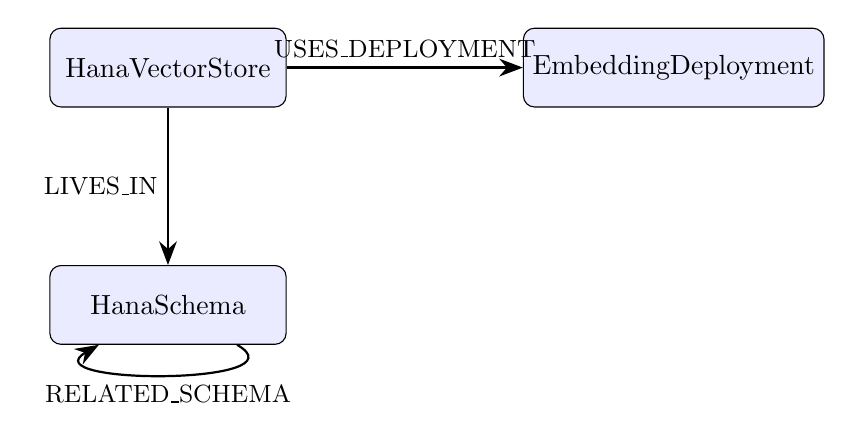
\begin{tikzpicture}[
  node distance=2.5cm,
  entity/.style={rectangle, draw, rounded corners, minimum width=3cm, minimum height=1cm, fill=blue!8},
  rel/.style={-{Stealth[length=3mm]}, thick}
]
  \node[entity] (vs) {HanaVectorStore};
  \node[entity, right=3cm of vs] (ed) {EmbeddingDeployment};
  \node[entity, below=2cm of vs] (hs) {HanaSchema};

  \draw[rel] (vs) -- node[above, font=\small] {USES\_DEPLOYMENT} (ed);
  \draw[rel] (vs) -- node[left, font=\small] {LIVES\_IN} (hs);
  \draw[rel] (hs) to[out=-30,in=-150,looseness=1.5] node[below, font=\small] {RELATED\_SCHEMA} (hs);
\end{tikzpicture}
\caption{KuzuDB entity-relationship diagram for the LangChain HANA store graph.}
\label{fig:kuzu-er}
\end{figure}

\subsection{OData Vocabularies Graph Schema}

The second graph schema models OData vocabulary metadata, with node
types \code{ODataVocabulary}, \code{VocabularyTerm}, and
\code{AnnotationTarget}.  Vocabulary terms are linked to their parent
vocabulary via \code{DEFINES\_TERM} edges, and annotation targets
reference terms via \code{ANNOTATED\_WITH} edges.  The OData MCP
endpoint (\code{odata\_mcp\_endpoint}, server.py line~300, default
\code{http://localhost:9150/mcp}) serves vocabulary lookups and is
integrated into the federated mesh as a preferred endpoint for the
\code{langchain\_load\_documents} tool (server.py lines~756--759).

\subsection{Cypher Query Tool with Write-Statement Blocking}

The \code{\_handle\_kuzu\_query} handler (server.py line~902) enforces
read-only access by blocking Cypher write statements:

\begin{lstlisting}[language=Python,caption={Write-statement blocking (server.py lines 906--909)},label=lst:cypher-block]
upper = cypher.upper().lstrip()
for disallowed in ("CREATE ", "MERGE ", "DELETE ",
                    "SET ", "REMOVE ", "DROP "):
    if upper.startswith(disallowed):
        return {"error":
            "Write Cypher statements are not permitted"
            " via this tool"}
\end{lstlisting}

\subsection{Graph Context Enrichment in RAG Chain}

The \code{\_handle\_langchain\_rag\_chain} method (server.py line~684) attaches
graph context from KuzuDB when the store factory is available
(lines~724--732):

\begin{lstlisting}[language=Python,caption={Graph context enrichment (server.py lines 723--732)},label=lst:graph-enrich]
# L4 -- attach graph context from KuzuDB when available
if _kuzu_store_factory is not None:
    try:
        store = _kuzu_store_factory()
        if store.available():
            ctx = store.get_store_context(table_name)
            if ctx:
                base["graphContext"] = ctx
    except Exception:
        pass
\end{lstlisting}

The \code{get\_store\_context} method (kuzu\_store.py line~196) traverses
\code{USES\_DEPLOYMENT} edges to return deployment metadata linked to
a vector store, providing the RAG chain with information about which
embedding model and resource group produced the vectors.


% ═══════════════════════════════════════════════════════════════════
\section{AI Core Configuration}
\label{sec:aicore}
% ═══════════════════════════════════════════════════════════════════

AI Core configuration is centralized in the MCP server's helper
functions (server.py lines~225--281).

\subsection{Token Caching with Expiry}

The module-level \code{\_cached\_token} dict (line~239) stores the OAuth2
token and its expiry timestamp.  The \code{get\_access\_token} function
(line~242) returns the cached token if still valid, otherwise performs a
fresh client credentials exchange:

\begin{lstlisting}[language=Python,caption={Token caching (server.py lines 239--263)},label=lst:token-cache]
_cached_token = {"token": None, "expires_at": 0}

def get_access_token(config):
    import time, base64
    if (_cached_token["token"]
        and time.time() < _cached_token["expires_at"]):
        return _cached_token["token"]
    ...
    auth = base64.b64encode(
        f"{config['client_id']}:{config['client_secret']}"
        .encode()).decode()
    req = urllib.request.Request(
        config["auth_url"],
        data=b"grant_type=client_credentials",
        headers={"Authorization": f"Basic {auth}", ...},
        method="POST")
    ...
    _cached_token["token"] = result["access_token"]
    _cached_token["expires_at"] = (
        time.time() + result.get("expires_in", 3600) - 60)
\end{lstlisting}

The 60-second pre-expiry buffer (line~260) prevents token-expired races.

\subsection{Resource Group Isolation}

Every AI Core request includes the \code{AI-Resource-Group} header
(server.py line~274), sourced from \code{AICORE\_RESOURCE\_GROUP}
(default \code{"default"}, line~231).  This enables tenant-level
isolation of deployments and model access.

\subsection{Deployment Discovery and Format Detection}

The chat handler (server.py line~582) fetches deployments via
\code{GET /v2/lm/deployments} and selects the first available.
Anthropic vs.\ OpenAI format detection occurs at line~587:

\begin{lstlisting}[language=Python,caption={Format detection (server.py lines 587--596)},label=lst:format-detect]
is_anthropic = "anthropic" in str(
    deployment.get("details", {})).lower()
...
if is_anthropic:
    result = aicore_request(config, "POST",
        f"/v2/inference/deployments/{deployment['id']}/invoke",
        {"anthropic_version": "bedrock-2023-05-31",
         "max_tokens": max_tokens, "messages": messages})
else:
    return aicore_request(config, "POST",
        f"/v2/inference/deployments/{deployment['id']}"
        "/chat/completions",
        {"messages": messages, "max_tokens": max_tokens})
\end{lstlisting}


% ═══════════════════════════════════════════════════════════════════
\section{Angular Fabric Console}
\label{sec:angular-console}
% ═══════════════════════════════════════════════════════════════════

The Angular Fabric Console provides a browser-based management interface
for the data fabric.  The core service is
\filepath{src/generativeUI/aifabric-webcomponents-ngx/apps/angular-shell/src/app/services/mcp.service.ts}.

\subsection{MCP Tool Invocation from Angular}

The \code{McpService} class (line~98) is a root-provided Angular service
that wraps MCP JSON-RPC calls in RxJS observables.  The private
\code{callTool} method (line~219) handles the full request lifecycle:

\begin{lstlisting}[language=Java,caption={Angular tool invocation (mcp.service.ts lines 219--229)},label=lst:angular-tool]
private callTool<T>(endpoint: string,
    toolName: string,
    args: Record<string, unknown>): Observable<T> {
  return this.mcpRequest<MCPToolResult>(
    endpoint, 'tools/call',
    { name: toolName, arguments: args }
  ).pipe(
    map(result => {
      const text = result.content?.[0]?.text;
      return text ? JSON.parse(text) : result;
    })
  );
}
\end{lstlisting}

Each request includes a correlation ID header (line~189) in the format
\code{console-\{timestamp\}-\{counter\}} and an optional Bearer token
(lines~191--193).

\subsection{Health Polling (30-Second Interval)}

Health polling is initialized in the constructor (line~124) and runs on
a 30-second RxJS \code{interval} (line~134):

\begin{lstlisting}[language=Java,caption={Health polling (mcp.service.ts lines 133--140)},label=lst:health-poll]
private startHealthPolling(): void {
  interval(30000).pipe(
    switchMap(() => this.checkAllHealth())
  ).subscribe();
  // Initial check
  this.checkAllHealth().subscribe();
}
\end{lstlisting}

The \code{checkAllHealth} method (line~142) uses \code{forkJoin} to
poll both the LangChain MCP (\code{/health}) and Streaming MCP
(\code{/health}) endpoints in parallel, computing an aggregate
health status.

\subsection{Deployment and Vector Store Management}

Deployment listing delegates to the streaming MCP's
\code{list\_deployments} tool (line~236).  Vector store operations use
the LangChain MCP:

\begin{itemize}
  \item \code{fetchVectorStores} (line~290) --- queries via
        \code{mangle\_query} with predicate \code{vector\_stores}.
  \item \code{createVectorStore} (line~308) --- calls
        \code{langchain\_vector\_store} tool.
  \item \code{addDocuments} (line~315) --- calls
        \code{langchain\_add\_documents} tool.
\end{itemize}

\subsection{Graph Queries}

KuzuDB access is exposed via two methods:

\begin{lstlisting}[language=Java,caption={KuzuDB graph methods (mcp.service.ts lines 365--382)},label=lst:angular-kuzu]
kuzuQuery(cypher: string,
    params?: Record<string, unknown>):
    Observable<{rows: unknown[]; rowCount: number}> {
  return this.callTool(this.langchainUrl, 'kuzu_query', {
    cypher,
    params: params ? JSON.stringify(params) : undefined
  });
}

kuzuIndex(entities: {
    vector_stores?: unknown[];
    deployments?: unknown[];
    schemas?: unknown[];
}): Observable<{stores_indexed: number; ...}> {
  return this.callTool(this.langchainUrl, 'kuzu_index', {
    vector_stores: JSON.stringify(
        entities.vector_stores || []),
    deployments: JSON.stringify(
        entities.deployments || []),
    schemas: JSON.stringify(entities.schemas || [])
  });
}
\end{lstlisting}

\subsection{Environment Configuration}

Development and production environments are configured separately in\\
\filepath{src/generativeUI/aifabric-webcomponents-ngx/apps/angular-shell/src/environments/}:

\begin{lstlisting}[language=Java,caption={Development environment (environment.ts lines 7--29)},label=lst:env-dev]
export const environment = {
  production: false,
  langchainMcpUrl: 'http://localhost:9140/mcp',
  streamingMcpUrl: 'http://localhost:9190/mcp',
  mcpAuthToken: '',
  hanaHost: '',
  hanaPort: 443,
  aiCoreBaseUrl: '',
  aiCoreResourceGroup: 'default',
  enableRag: true,
  enableStreaming: true,
  enableKuzuGraph: true,
};
\end{lstlisting}

In production (environment.prod.ts line~3), URLs are resolved from a
runtime configuration object: \code{(window as any).\_\_SAP\_CONFIG\_\_?.langchainMcpUrl || '/api/langchain/mcp'}.


% ═══════════════════════════════════════════════════════════════════
\section{OData Vocabularies Integration}
\label{sec:odata}
% ═══════════════════════════════════════════════════════════════════

The OData vocabulary integration enables the data fabric to understand
and query SAP OData service metadata, annotations, and vocabulary terms.

\subsection{Vocabulary Discovery}

The MCP server's fact store includes an OData vocabulary MCP endpoint
(server.py line~299--301), registered as \code{odata-vocab-mcp} in the
service registry (line~526).  The endpoint listens on port 9150 by default
and provides term lookups, annotation target resolution, and schema
relationship queries.

\subsection{Federated Document Loading with OData Context}

The \code{\_handle\_langchain\_load\_documents} handler (server.py line~750)
delegates to the OData MCP endpoint when loading documents, requesting
annotation context:

\begin{lstlisting}[language=Python,caption={OData-enriched document loading (server.py lines 756--768)},label=lst:odata-load]
delegation = self._federated_mcp_call(
    "get_rag_context",
    {"query": source,
     "include_annotations": loader_type != "text"},
    preferred=[self.odata_mcp_endpoint],
)
if delegation:
    return {
        "source": source,
        "loader_type": loader_type,
        "status": "federated",
        "federated_source": delegation["source"],
        "result": delegation["result"],
    }
\end{lstlisting}

\subsection{Schema Relationships in the Graph}

OData vocabulary relationships are modeled in the KuzuDB graph via the
\code{HanaSchema} node type and \code{RELATED\_SCHEMA} edges
(kuzu\_store.py lines~82--85).  Schema nodes carry a
\code{classification} property (\code{internal}, \code{public}, etc.)
that can be queried via Cypher:

\begin{lstlisting}[language=Python,caption={Schema context query (kuzu\_store.py lines 208--217)},label=lst:schema-ctx]
def get_schema_context(self, schema_id):
    return self.run_query(
        "MATCH (s:HanaVectorStore)"
        "-[:LIVES_IN]->(h:HanaSchema {schemaId: $id}) "
        "RETURN s.storeId AS storeId, "
        "s.tableName AS tableName, "
        "s.embeddingModel AS embeddingModel, "
        "'lives_in' AS relation",
        {"id": schema_id},
    )
\end{lstlisting}

\subsection{Mangle-Based Term Lookup}

The \code{mangle\_query} tool (server.py line~804) supports OData
vocabulary predicates by delegating to both the HANA and OData MCP
endpoints with \code{preferred=[self.hana\_mcp\_endpoint, self.odata\_mcp\_endpoint]}
(line~816).  This enables queries like
\code{mangle\_query(predicate="vocabulary\_term", args=["Org.OData.Core.V1"])}
to resolve vocabulary definitions.


% ═══════════════════════════════════════════════════════════════════
\section{Telemetry and Observability}
\label{sec:telemetry}
% ═══════════════════════════════════════════════════════════════════

The data fabric implements comprehensive OpenTelemetry tracing across
both the CAP LLM Plugin and the MCP server.

\subsection{OpenTelemetry Tracer with Graceful Degradation}

The tracer factory in
\filepath{src/data/cap-llm-plugin-main/src/telemetry/tracer.ts}
(lines~81--105) provides a thin wrapper that degrades to no-op stubs
when \code{@opentelemetry/api} is not installed:

\begin{lstlisting}[language=Java,caption={Tracer factory (tracer.ts lines 81--105)},label=lst:tracer]
export function getTracer(): PluginTracer {
  if (_cachedTracer !== null) return _cachedTracer;
  try {
    const otelApi = require("@opentelemetry/api");
    const realTracer = otelApi.trace.getTracer(
        TRACER_NAME, TRACER_VERSION);
    _cachedTracer = {
      startSpan: (name) => {
        const span = realTracer.startSpan(name);
        return {
          setAttribute: (key, value) =>
            { span.setAttribute(key, value); },
          addEvent: (name, attrs) =>
            { span.addEvent(name, attrs); },
          recordException: (err) =>
            { span.recordException(err); },
          setStatus: (status) =>
            { span.setStatus(status); },
          end: () => { span.end(); },
        };
      },
    };
  } catch {
    _cachedTracer = noopTracer;
  }
  return _cachedTracer;
}
\end{lstlisting}

The \code{SpanStatusCode} constants (line~55) mirror \code{@opentelemetry/api}
values: \code{UNSET=0}, \code{OK=1}, \code{ERROR=2}.

\subsection{OTEL Middleware for SDK Calls}

The \code{createOtelMiddleware} function in
\filepath{src/data/cap-llm-plugin-main/src/telemetry/ai-sdk-middleware.ts}
(line~79) wraps \code{@sap-cloud-sdk/http-client} requests in
OpenTelemetry spans and injects W3C Trace Context headers
(\code{traceparent}, \code{tracestate}) for distributed tracing:

\begin{lstlisting}[language=Java,caption={OTEL middleware (ai-sdk-middleware.ts lines 79--143)},label=lst:otel-mw]
export function createOtelMiddleware(
    options: OtelMiddlewareOptions = {}): AiSdkMiddleware {
  return function otelMiddleware(middlewareOptions) {
    return async function otelMiddlewareHandler(requestConfig) {
      const span = getTracer().startSpan(spanName);
      span.setAttribute("http.method", "POST");
      if (options.endpoint)
        span.setAttribute("ai_core.endpoint",
            options.endpoint);
      if (options.resourceGroup)
        span.setAttribute("ai_core.resource_group",
            options.resourceGroup);
      ...
      const enrichedConfig =
          injectTraceContext(requestConfig);
      span.addEvent("ai_core.request_sent");
      try {
        const response =
            await middlewareOptions.fn(enrichedConfig);
        span.setAttribute("http.status_code",
            response.status);
        ...
      } catch (e) {
        span.recordException(e);
        span.setStatus({code: SpanStatusCode.ERROR, ...});
        throw e;
      } finally { span.end(); }
    };
  };
}
\end{lstlisting}

\subsection{Span Attributes}

Table~\ref{tab:span-attrs} lists the key span attributes emitted
across the data fabric.

\begin{longtable}{@{}llp{5cm}@{}}
\caption{OpenTelemetry span attributes}
\label{tab:span-attrs} \\
\toprule
\textbf{Attribute} & \textbf{Source File} & \textbf{Description} \\
\midrule
\endfirsthead
\toprule
\textbf{Attribute} & \textbf{Source File} & \textbf{Description} \\
\midrule
\endhead
\bottomrule
\endlastfoot
\code{llm.embedding.model}          & cap-llm-plugin.ts:246  & Embedding model name \\
\code{llm.resource\_group}          & cap-llm-plugin.ts:247  & AI Core resource group \\
\code{llm.chat.model}               & cap-llm-plugin.ts:317  & Chat completion model name \\
\code{db.hana.table}                & cap-llm-plugin.ts:452  & HANA table for vector ops \\
\code{db.hana.algo}                 & cap-llm-plugin.ts:453  & Similarity algorithm \\
\code{db.hana.top\_k}               & cap-llm-plugin.ts:668  & Number of results requested \\
\code{db.hana.embedding\_dims}      & cap-llm-plugin.ts:669  & Embedding vector dimensions \\
\code{llm.usage.total\_tokens}      & cap-llm-plugin.ts:363  & Total tokens consumed \\
\code{llm.usage.prompt\_tokens}     & cap-llm-plugin.ts:361  & Input tokens consumed \\
\code{llm.usage.completion\_tokens} & cap-llm-plugin.ts:362  & Output tokens consumed \\
\code{rag.min\_score}               & cap-llm-plugin.ts:497  & Minimum similarity score \\
\code{rag.max\_score}               & cap-llm-plugin.ts:498  & Maximum similarity score \\
\code{rag.context\_chars}           & cap-llm-plugin.ts:532  & Characters of context used \\
\code{rag.documents\_used}          & cap-llm-plugin.ts:534  & Number of documents in context \\
\code{ai\_core.endpoint}            & ai-sdk-middleware.ts:93 & AI Core API endpoint path \\
\code{ai\_core.resource\_group}     & ai-sdk-middleware.ts:96 & Resource group for isolation \\
\code{http.status\_code}            & ai-sdk-middleware.ts:117 & HTTP response status code \\
\code{anonymization.entity}         & cap-llm-plugin.ts:146  & Entity name for anonymization \\
\code{content\_filter.type}         & cap-llm-plugin.ts:1005 & Content filter provider type \\
\end{longtable}

\subsection{Event Logging}

In addition to span attributes, the system emits structured events
within spans.  Key events include \code{embedding\_response\_received},
\code{similarity\_search\_completed} (with \code{search.result\_count}
and \code{search.method}), \code{chat\_completion\_response\_received},
\code{stream\_started}, \code{stream\_completed} (with
\code{stream.finish\_reason} and \code{stream.total\_tokens}),
\code{anonymized\_data\_fetched}, and \code{quality\_warnings}.


% ═══════════════════════════════════════════════════════════════════
\section{Security}
\label{sec:security}
% ═══════════════════════════════════════════════════════════════════

The data fabric implements defense-in-depth security across network,
input validation, and content safety layers.

\subsection{CORS with Explicit Origin Allowlist}

The MCP server uses an explicit origin allowlist (server.py lines~29--32)
rather than wildcard CORS:

\begin{lstlisting}[language=Python,caption={CORS allowlist (server.py lines 29--39)},label=lst:cors]
CORS_ALLOWED_ORIGINS = [
    o.strip() for o in os.environ.get(
        "CORS_ALLOWED_ORIGINS",
        "http://localhost:3000,"
        "http://127.0.0.1:3000").split(",")
    if o.strip()
]

def _cors_origin(handler):
    origin = (handler.headers.get("Origin") or "").strip()
    if origin and origin in CORS_ALLOWED_ORIGINS:
        return origin
    return CORS_ALLOWED_ORIGINS[0] \
        if CORS_ALLOWED_ORIGINS else None
\end{lstlisting}

\subsection{Request Size Limits}

The \code{MAX\_REQUEST\_BYTES} constant (server.py line~42, default
1\,MB) is enforced in the HTTP handler (line~1035):

\begin{lstlisting}[language=Python,caption={Request size check (server.py lines 1034--1037)},label=lst:max-request]
if content_length > MAX_REQUEST_BYTES:
    self._write_json(413, {
        "jsonrpc": "2.0", "id": None,
        "error": {"code": -32600,
                  "message": "Request too large"}})
    return
\end{lstlisting}

\subsection{SQL Identifier Validation}

The \code{validateSqlIdentifier} function in
\filepath{src/data/cap-llm-plugin-main/lib/validation-utils.js}
(lines~9--29) uses a strict regex to prevent SQL injection in
identifier positions:

\begin{lstlisting}[language=Java,caption={SQL identifier validation (validation-utils.js lines 9--29)},label=lst:sql-valid]
const VALID_SQL_IDENTIFIER = /^[A-Za-z_][A-Za-z0-9_-]*$/;

function validateSqlIdentifier(name, label) {
  if (typeof name !== "string" || name.length === 0) {
    throw new Error(`Invalid ${label}: must be a `
        + `non-empty string.`);
  }
  if (!VALID_SQL_IDENTIFIER.test(name)) {
    throw new Error(
      `Invalid ${label}: "${name}" contains characters `
      + `that are not allowed in SQL identifiers.`);
  }
}
\end{lstlisting}

\subsection{Embedding Vector Validation}

The \code{validateEmbeddingVector} function (validation-utils.js
lines~54--66) ensures embeddings are non-empty arrays of finite numbers,
preventing NaN or Infinity values from reaching HANA:

\begin{lstlisting}[language=Java,caption={Embedding validation (validation-utils.js lines 54--66)},label=lst:embed-valid]
function validateEmbeddingVector(embedding) {
  if (!Array.isArray(embedding)
      || embedding.length === 0) {
    throw new Error("Invalid embedding: must be a "
        + "non-empty array.");
  }
  for (let i = 0; i < embedding.length; i++) {
    if (typeof embedding[i] !== "number"
        || !isFinite(embedding[i])) {
      throw new Error(
        `Invalid embedding: element at index ${i} `
        + `is not a finite number.`);
    }
  }
}
\end{lstlisting}

Additionally, \code{validateEmbeddingDimensions} (line~104) cross-references
a known model dimensions table to detect model-mismatch bugs where query
and index embeddings use different models.

\subsection{Content Safety Filters}

The \code{getContentFilters} method (cap-llm-plugin.ts line~1003)
constructs Azure Content Safety filters via the \code{@sap-ai-sdk/orchestration}
SDK.  Only the \code{"azure"} type is currently supported (line~1008),
and unsupported types produce a structured \code{ChatCompletionError}
with code \code{UNSUPPORTED\_FILTER\_TYPE}.

The AG-UI agent service (\filepath{src/data/cap-llm-plugin-main/srv/ag-ui/agent-service.ts})
implements additional security via intent routing (line~158), which can
block requests entirely (returning HTTP 403) when the \code{IntentRouter}
classifies the user message as policy-violating (lines~171--181).


% ═══════════════════════════════════════════════════════════════════
\section{Architecture Topology}
\label{sec:topology}
% ═══════════════════════════════════════════════════════════════════

Figure~\ref{fig:topology} illustrates the overall data fabric topology,
showing the relationships between the MCP servers, the CAP LLM Plugin,
the Angular console, and the backend services.

\begin{figure}[h]
\centering
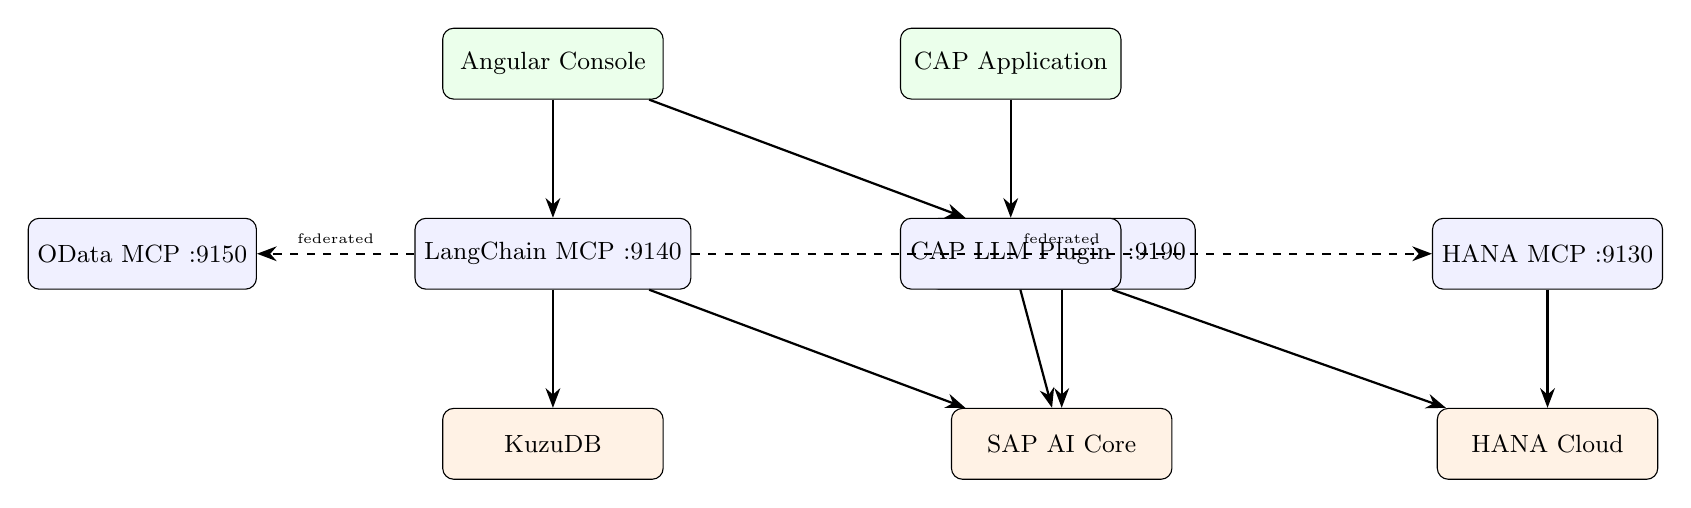
\begin{tikzpicture}[
  node distance=1.8cm and 2.5cm,
  svc/.style={rectangle, draw, rounded corners=4pt, minimum width=2.8cm, minimum height=0.9cm, font=\small, fill=blue!6},
  ext/.style={rectangle, draw, rounded corners=4pt, minimum width=2.8cm, minimum height=0.9cm, font=\small, fill=orange!10},
  cli/.style={rectangle, draw, rounded corners=4pt, minimum width=2.8cm, minimum height=0.9cm, font=\small, fill=green!8},
  arr/.style={-{Stealth[length=2.5mm]}, thick},
  darr/.style={-{Stealth[length=2.5mm]}, thick, dashed}
]
  % Clients
  \node[cli] (console) {Angular Console};
  \node[cli, right=3cm of console] (capapp) {CAP Application};

  % MCP Servers
  \node[svc, below=1.5cm of console] (lcmcp) {LangChain MCP :9140};
  \node[svc, right=3cm of lcmcp] (strmcp) {Streaming MCP :9190};
  \node[svc, left=2cm of lcmcp] (odatamcp) {OData MCP :9150};
  \node[svc, right=3cm of strmcp] (hanamcp) {HANA MCP :9130};

  % Backend
  \node[ext, below=1.5cm of lcmcp] (kuzu) {KuzuDB};
  \node[ext, below=1.5cm of strmcp] (aicore) {SAP AI Core};
  \node[ext, below=1.5cm of hanamcp] (hana) {HANA Cloud};

  % Plugin
  \node[svc, below=1.5cm of capapp] (plugin) {CAP LLM Plugin};

  % Arrows
  \draw[arr] (console) -- (lcmcp);
  \draw[arr] (console) -- (strmcp);
  \draw[arr] (capapp) -- (plugin);
  \draw[arr] (plugin) -- (aicore);
  \draw[arr] (plugin) -- (hana);
  \draw[arr] (lcmcp) -- (kuzu);
  \draw[darr] (lcmcp) -- node[above,font=\tiny] {federated} (hanamcp);
  \draw[darr] (lcmcp) -- node[above,font=\tiny] {federated} (odatamcp);
  \draw[arr] (strmcp) -- (aicore);
  \draw[arr] (hanamcp) -- (hana);
  \draw[arr] (lcmcp) -- (aicore);
\end{tikzpicture}
\caption{Data fabric topology showing MCP servers, backend services,
and client applications.  Dashed arrows represent federated MCP calls.}
\label{fig:topology}
\end{figure}


% ═══════════════════════════════════════════════════════════════════
\section{Summary of Configuration Constants}
\label{sec:constants}
% ═══════════════════════════════════════════════════════════════════

Table~\ref{tab:constants} summarizes the environment-configurable
constants that govern the data fabric's behavior.

\begin{longtable}{@{}llrl@{}}
\caption{Configuration constants (server.py lines 42--48)}
\label{tab:constants} \\
\toprule
\textbf{Constant} & \textbf{Env Var} & \textbf{Default} & \textbf{Purpose} \\
\midrule
\endfirsthead
\toprule
\textbf{Constant} & \textbf{Env Var} & \textbf{Default} & \textbf{Purpose} \\
\midrule
\endhead
\bottomrule
\endlastfoot
\code{MAX\_REQUEST\_BYTES}       & \code{MCP\_MAX\_REQUEST\_BYTES}    & 1\,048\,576 & Request body size limit \\
\code{MAX\_TOOL\_TOKENS}         & \code{MCP\_MAX\_TOOL\_TOKENS}      & 8192        & Max tokens per tool call \\
\code{MAX\_TOP\_K}               & \code{MCP\_MAX\_TOP\_K}            & 100         & Max similarity results \\
\code{MAX\_DOCS\_PER\_CALL}      & \code{MCP\_MAX\_DOCS\_PER\_CALL}   & 1000        & Max documents per add call \\
\code{MAX\_CHUNK\_SIZE}          & \code{MCP\_MAX\_CHUNK\_SIZE}       & 4000        & Max text chunk size (chars) \\
\code{MAX\_REMOTE\_ENDPOINTS}    & \code{MCP\_MAX\_REMOTE\_ENDPOINTS} & 25          & Max federated endpoints \\
\code{REMOTE\_MCP\_TIMEOUT}      & \code{MCP\_REMOTE\_TIMEOUT\_SECONDS} & 3         & Federated call timeout (s) \\
\end{longtable}


% ═══════════════════════════════════════════════════════════════════
\section{Conclusion}
\label{sec:conclusion}
% ═══════════════════════════════════════════════════════════════════

The SAP OSS Data Fabric architecture achieves several design goals:

\begin{enumerate}
  \item \textbf{Protocol uniformity} --- All services communicate via
        JSON-RPC 2.0 over HTTP, enabling language-agnostic tool invocation
        from Python, TypeScript, and Angular clients.

  \item \textbf{Federated discovery} --- The MCP mesh automatically discovers
        and delegates to peer servers, with priority ordering and graceful
        fallback when remote endpoints are unavailable.

  \item \textbf{Defense in depth} --- Security is enforced at multiple layers:
        CORS origin allowlists, request size limits, SQL identifier validation,
        embedding vector validation, content safety filters, and intent-based
        request blocking.

  \item \textbf{Observability} --- OpenTelemetry tracing with graceful
        degradation provides comprehensive span attributes across embedding,
        chat, RAG, and streaming operations without requiring OTel as a
        hard dependency.

  \item \textbf{Graph-enriched RAG} --- KuzuDB provides structural context
        about vector store relationships, embedding deployments, and schema
        classifications that augment the retrieval-augmented generation
        pipeline.

  \item \textbf{CDS contract enforcement} --- The CDS service definition
        in \code{llm-service.cds} serves as the single source of truth for
        the plugin's typed API, with automated contract drift detection
        and OpenAPI spec generation.
\end{enumerate}

\end{document}
